\section{小结}

\begin{frame}
  \frametitle{小结}
  \begin{enumerate}
    \item 介绍了机器人定位、分类、方法。
    \item 介绍了AMCL算法
    \item 机器人运动模型和在AMCL中的实现及参数意义
    \item 机器人Lader感知模型和在AMCL中的实现及参数意义
  \end{enumerate}
  
\end{frame}

\begin{frame}
  \frametitle{推荐阅读书籍}
  \begin{columns}
    \column{0.5\textwidth}
    \begin{enumerate}
      \item 《概率机器人》
      \item 《机器人学中的状态估计》
      \item 《视觉SLAM十四讲》
      \item 《概率图模型原理与技术》
      \item 《凸优化》
    \end{enumerate}
    \column{0.5\textwidth}
    \begin{figure}
      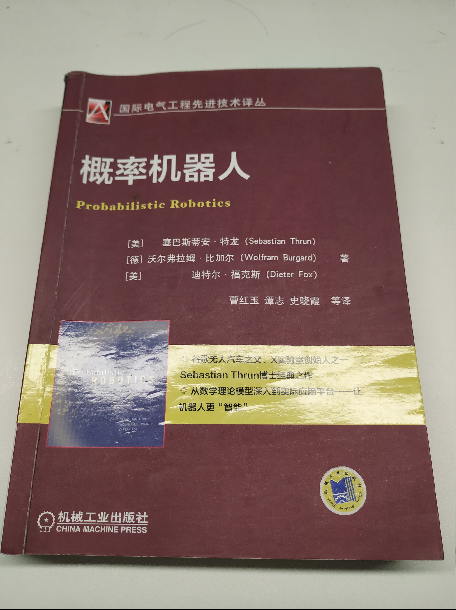
\includegraphics[height=2.5cm]{amcl/refbook1.png}
      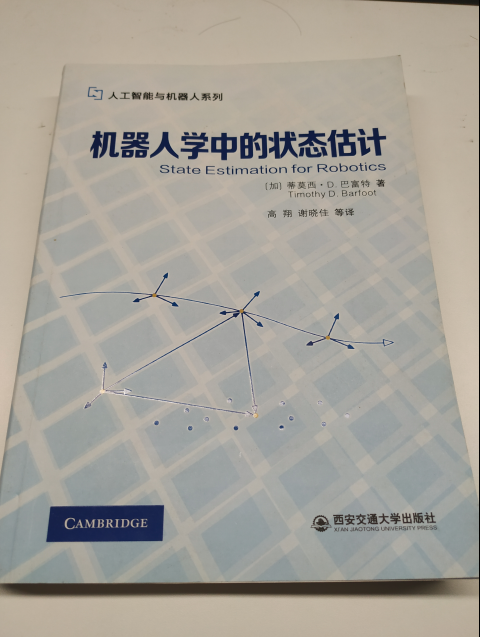
\includegraphics[height=2.5cm]{amcl/refbook2.png}
      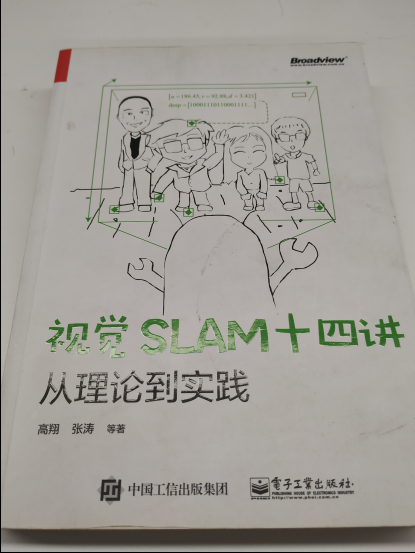
\includegraphics[height=2.5cm]{amcl/refbook4.png}

      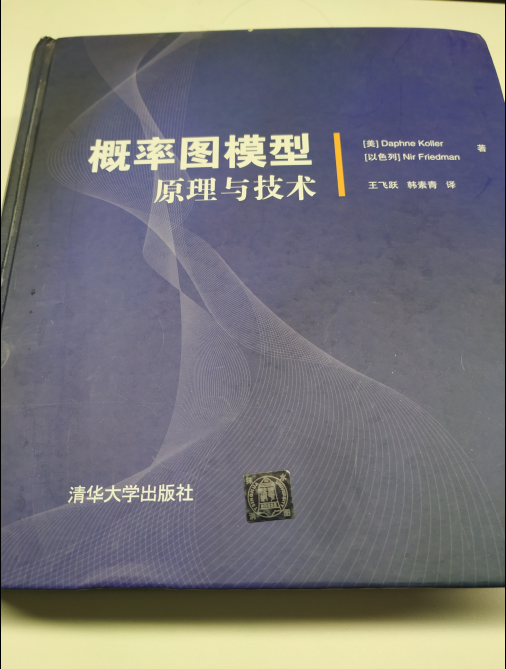
\includegraphics[height=2.5cm]{amcl/refbook3.png}
      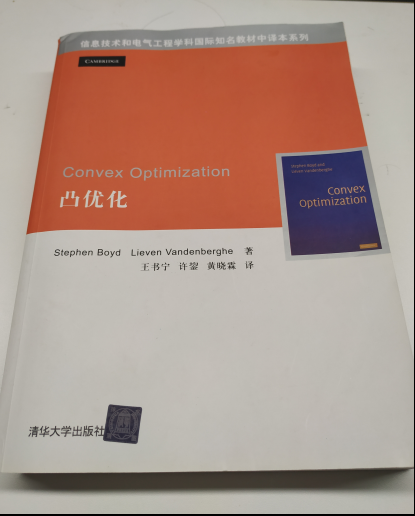
\includegraphics[height=2.5cm]{amcl/refbook5.png}
    \end{figure}
  \end{columns}

  
\end{frame}

% \begin{frame}
%   \begin{figure}
%     % 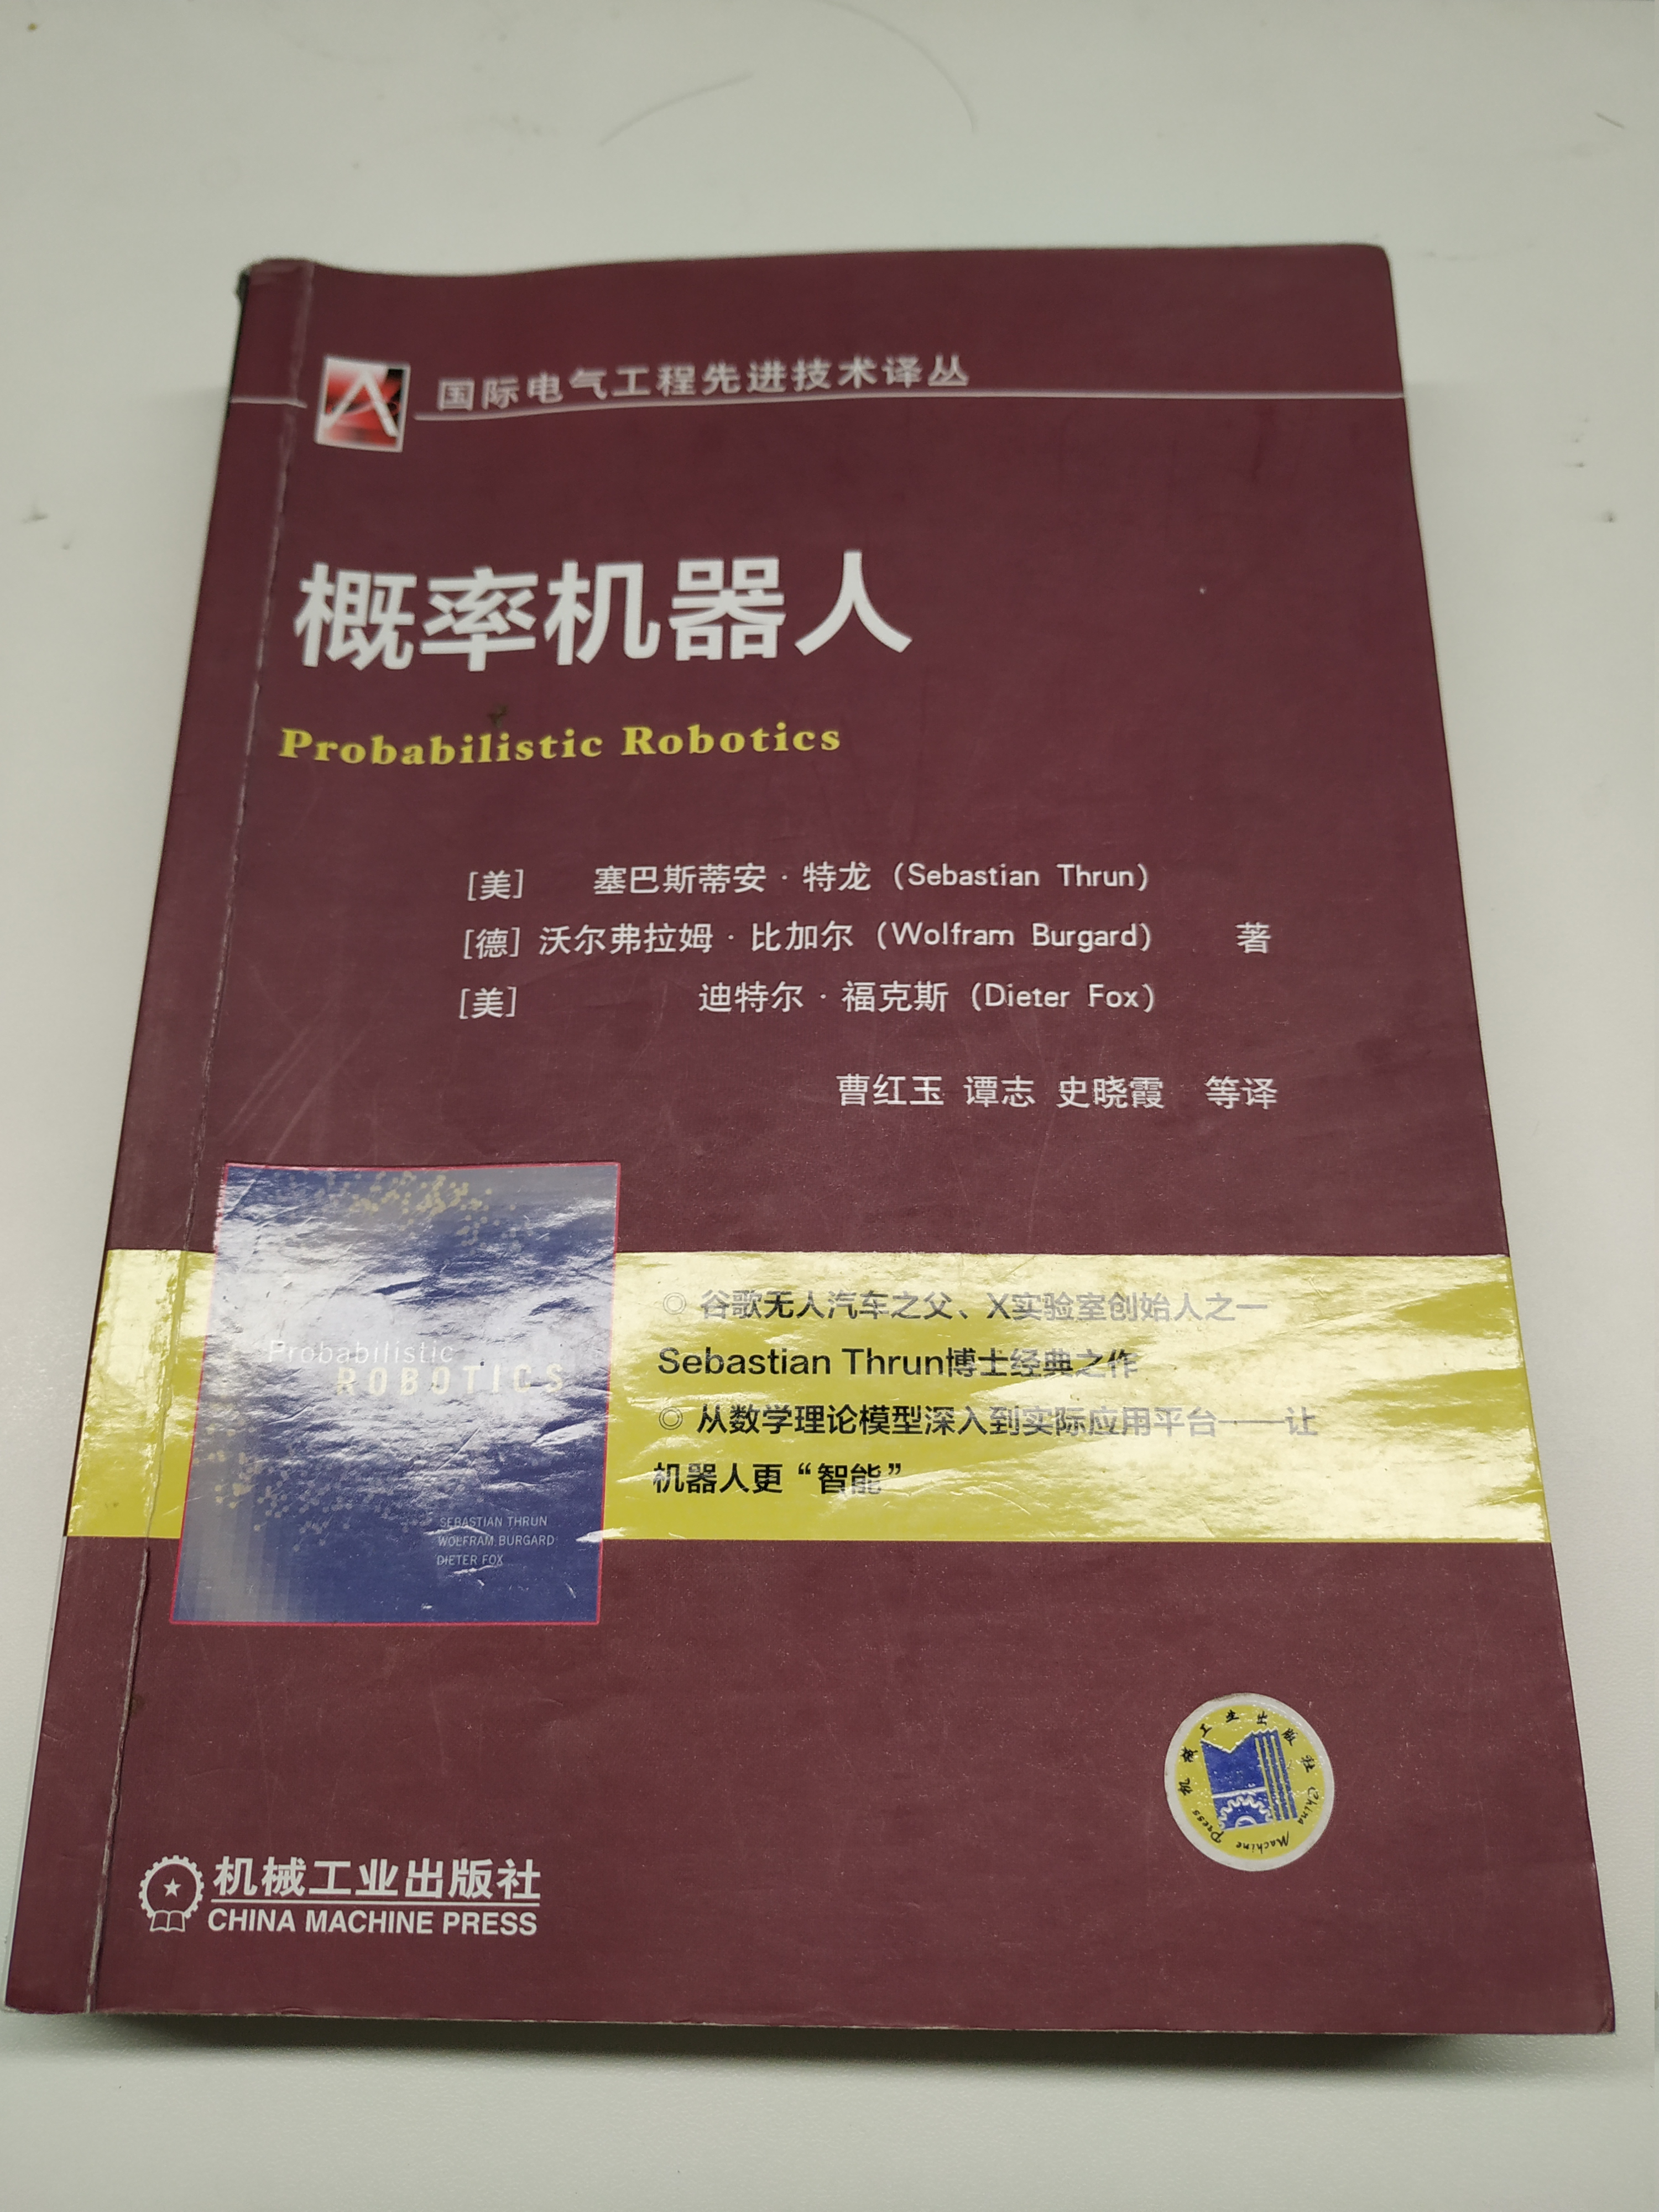
\includegraphics[height=3.0cm]{amcl/gljqr.jpg}
%     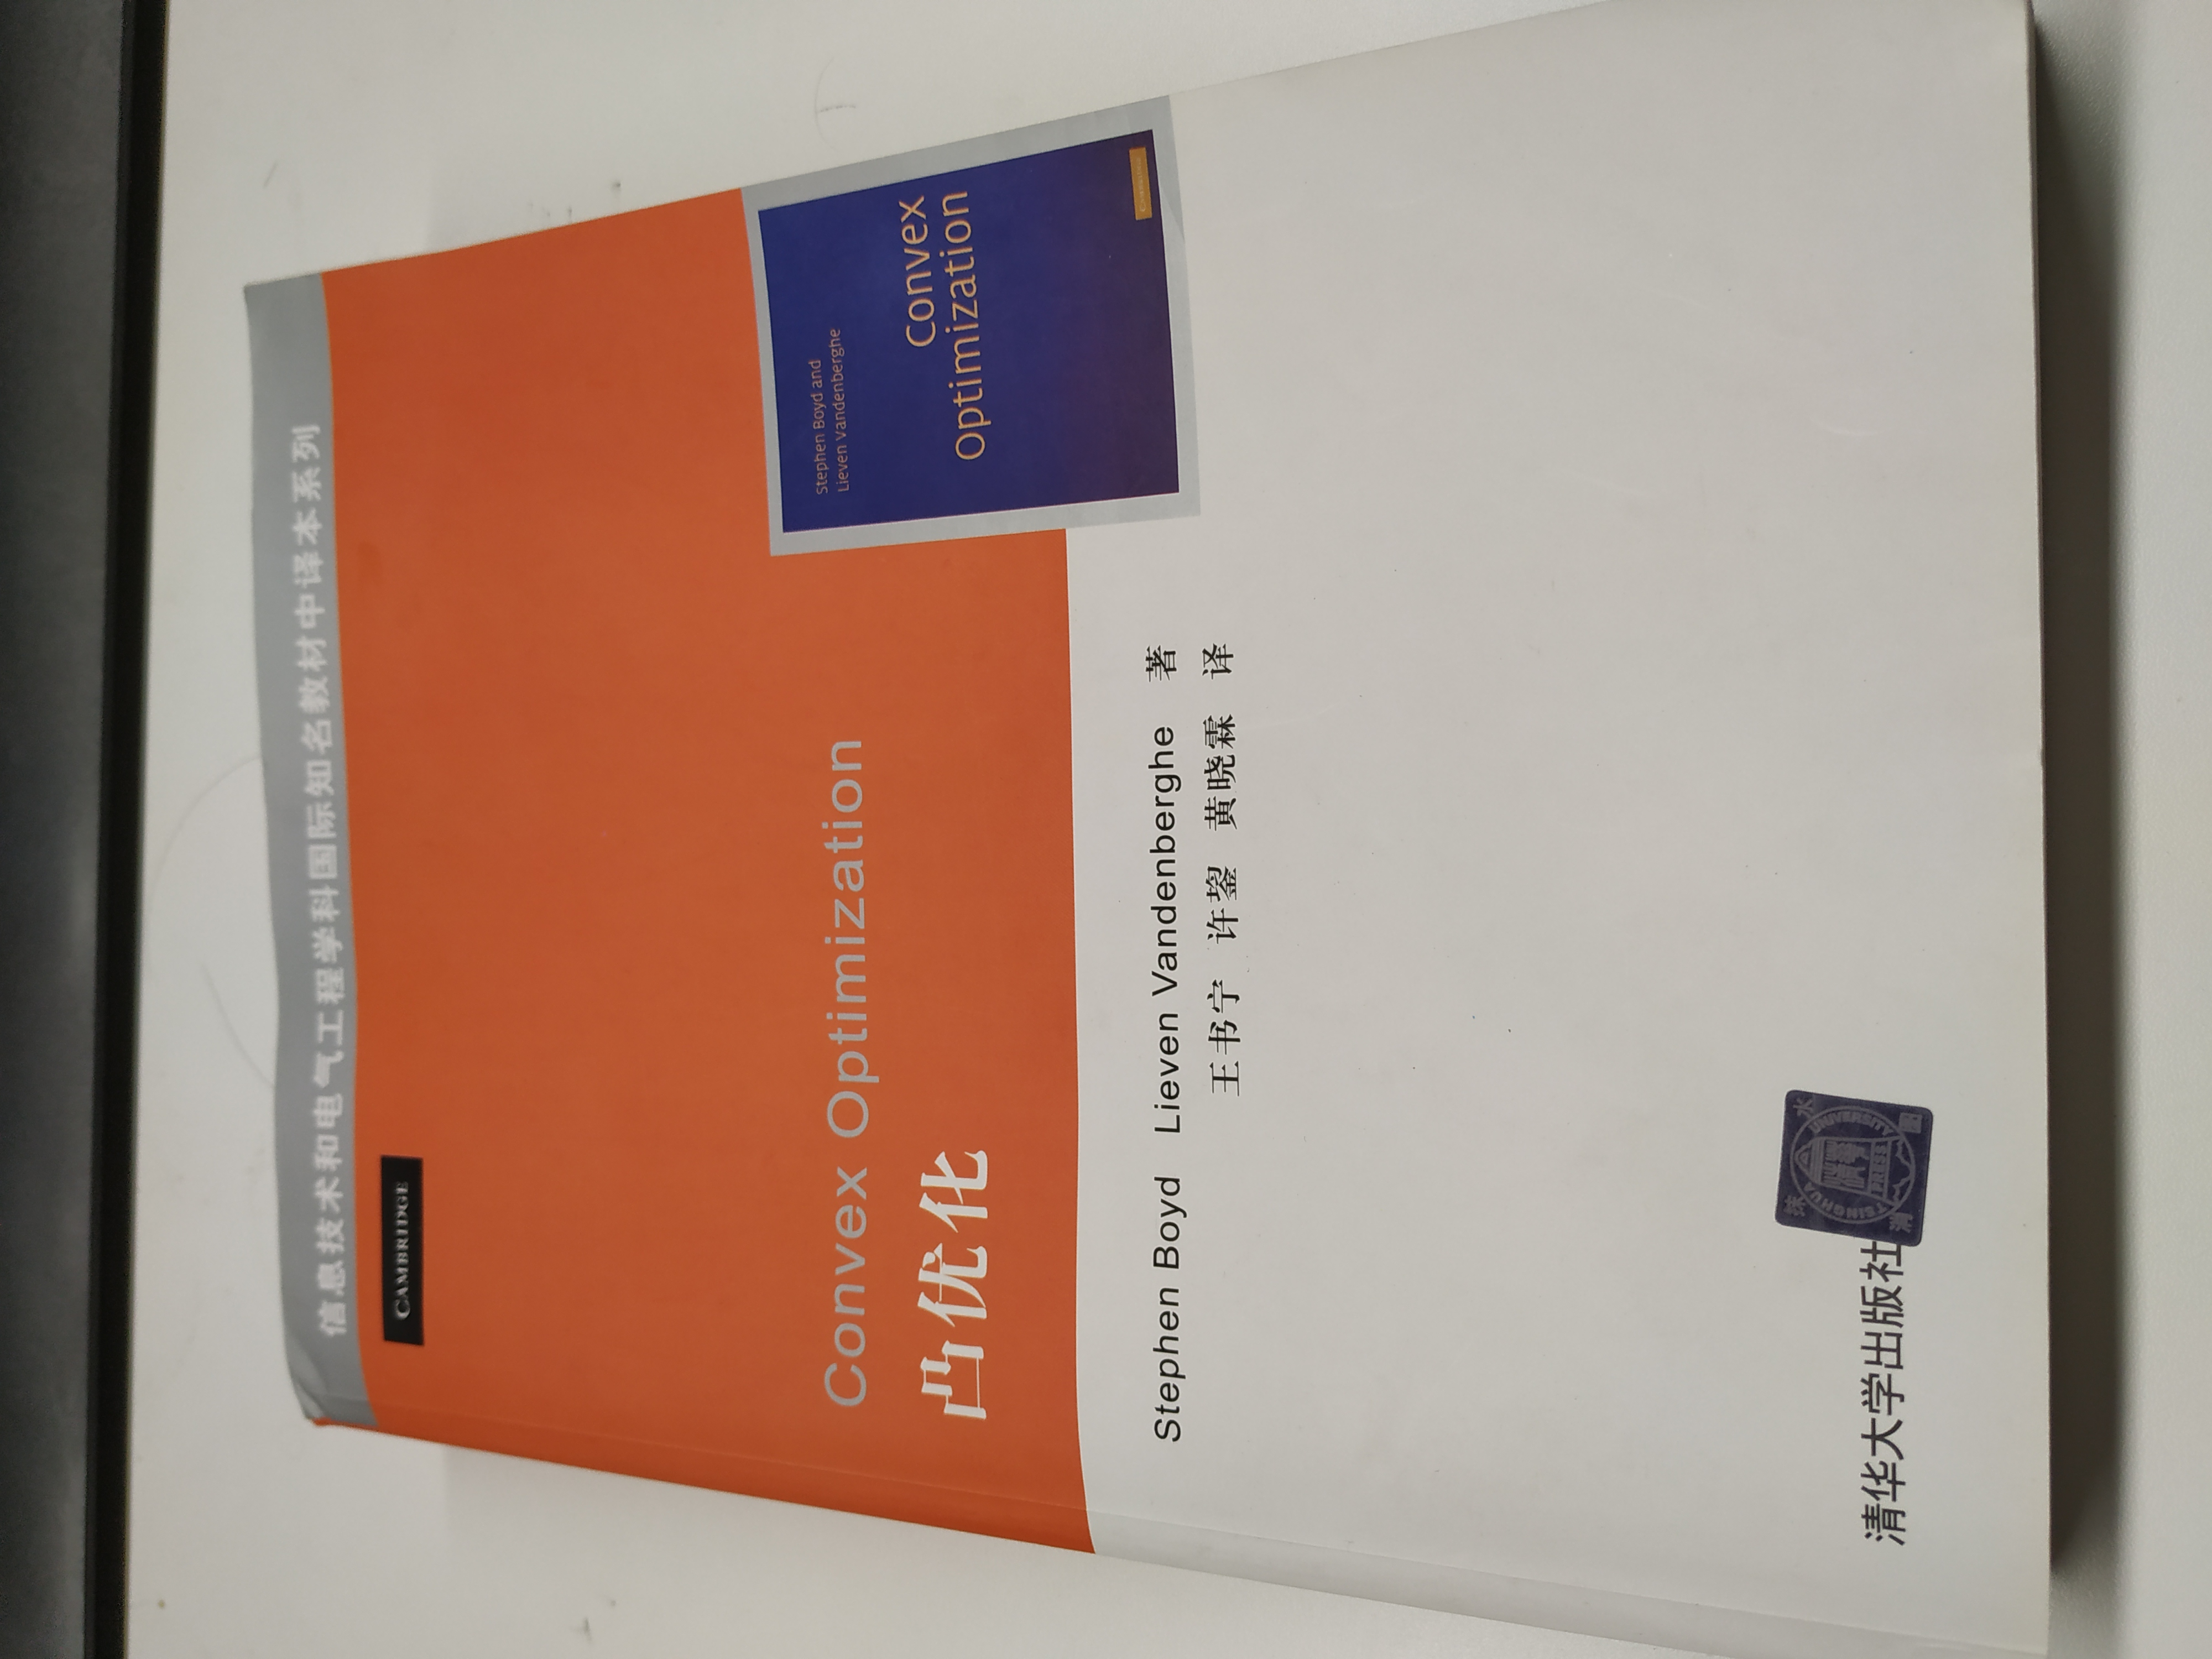
\includegraphics[width=2.5cm,height=3.5cm]{amcl/tyh.jpg}
%     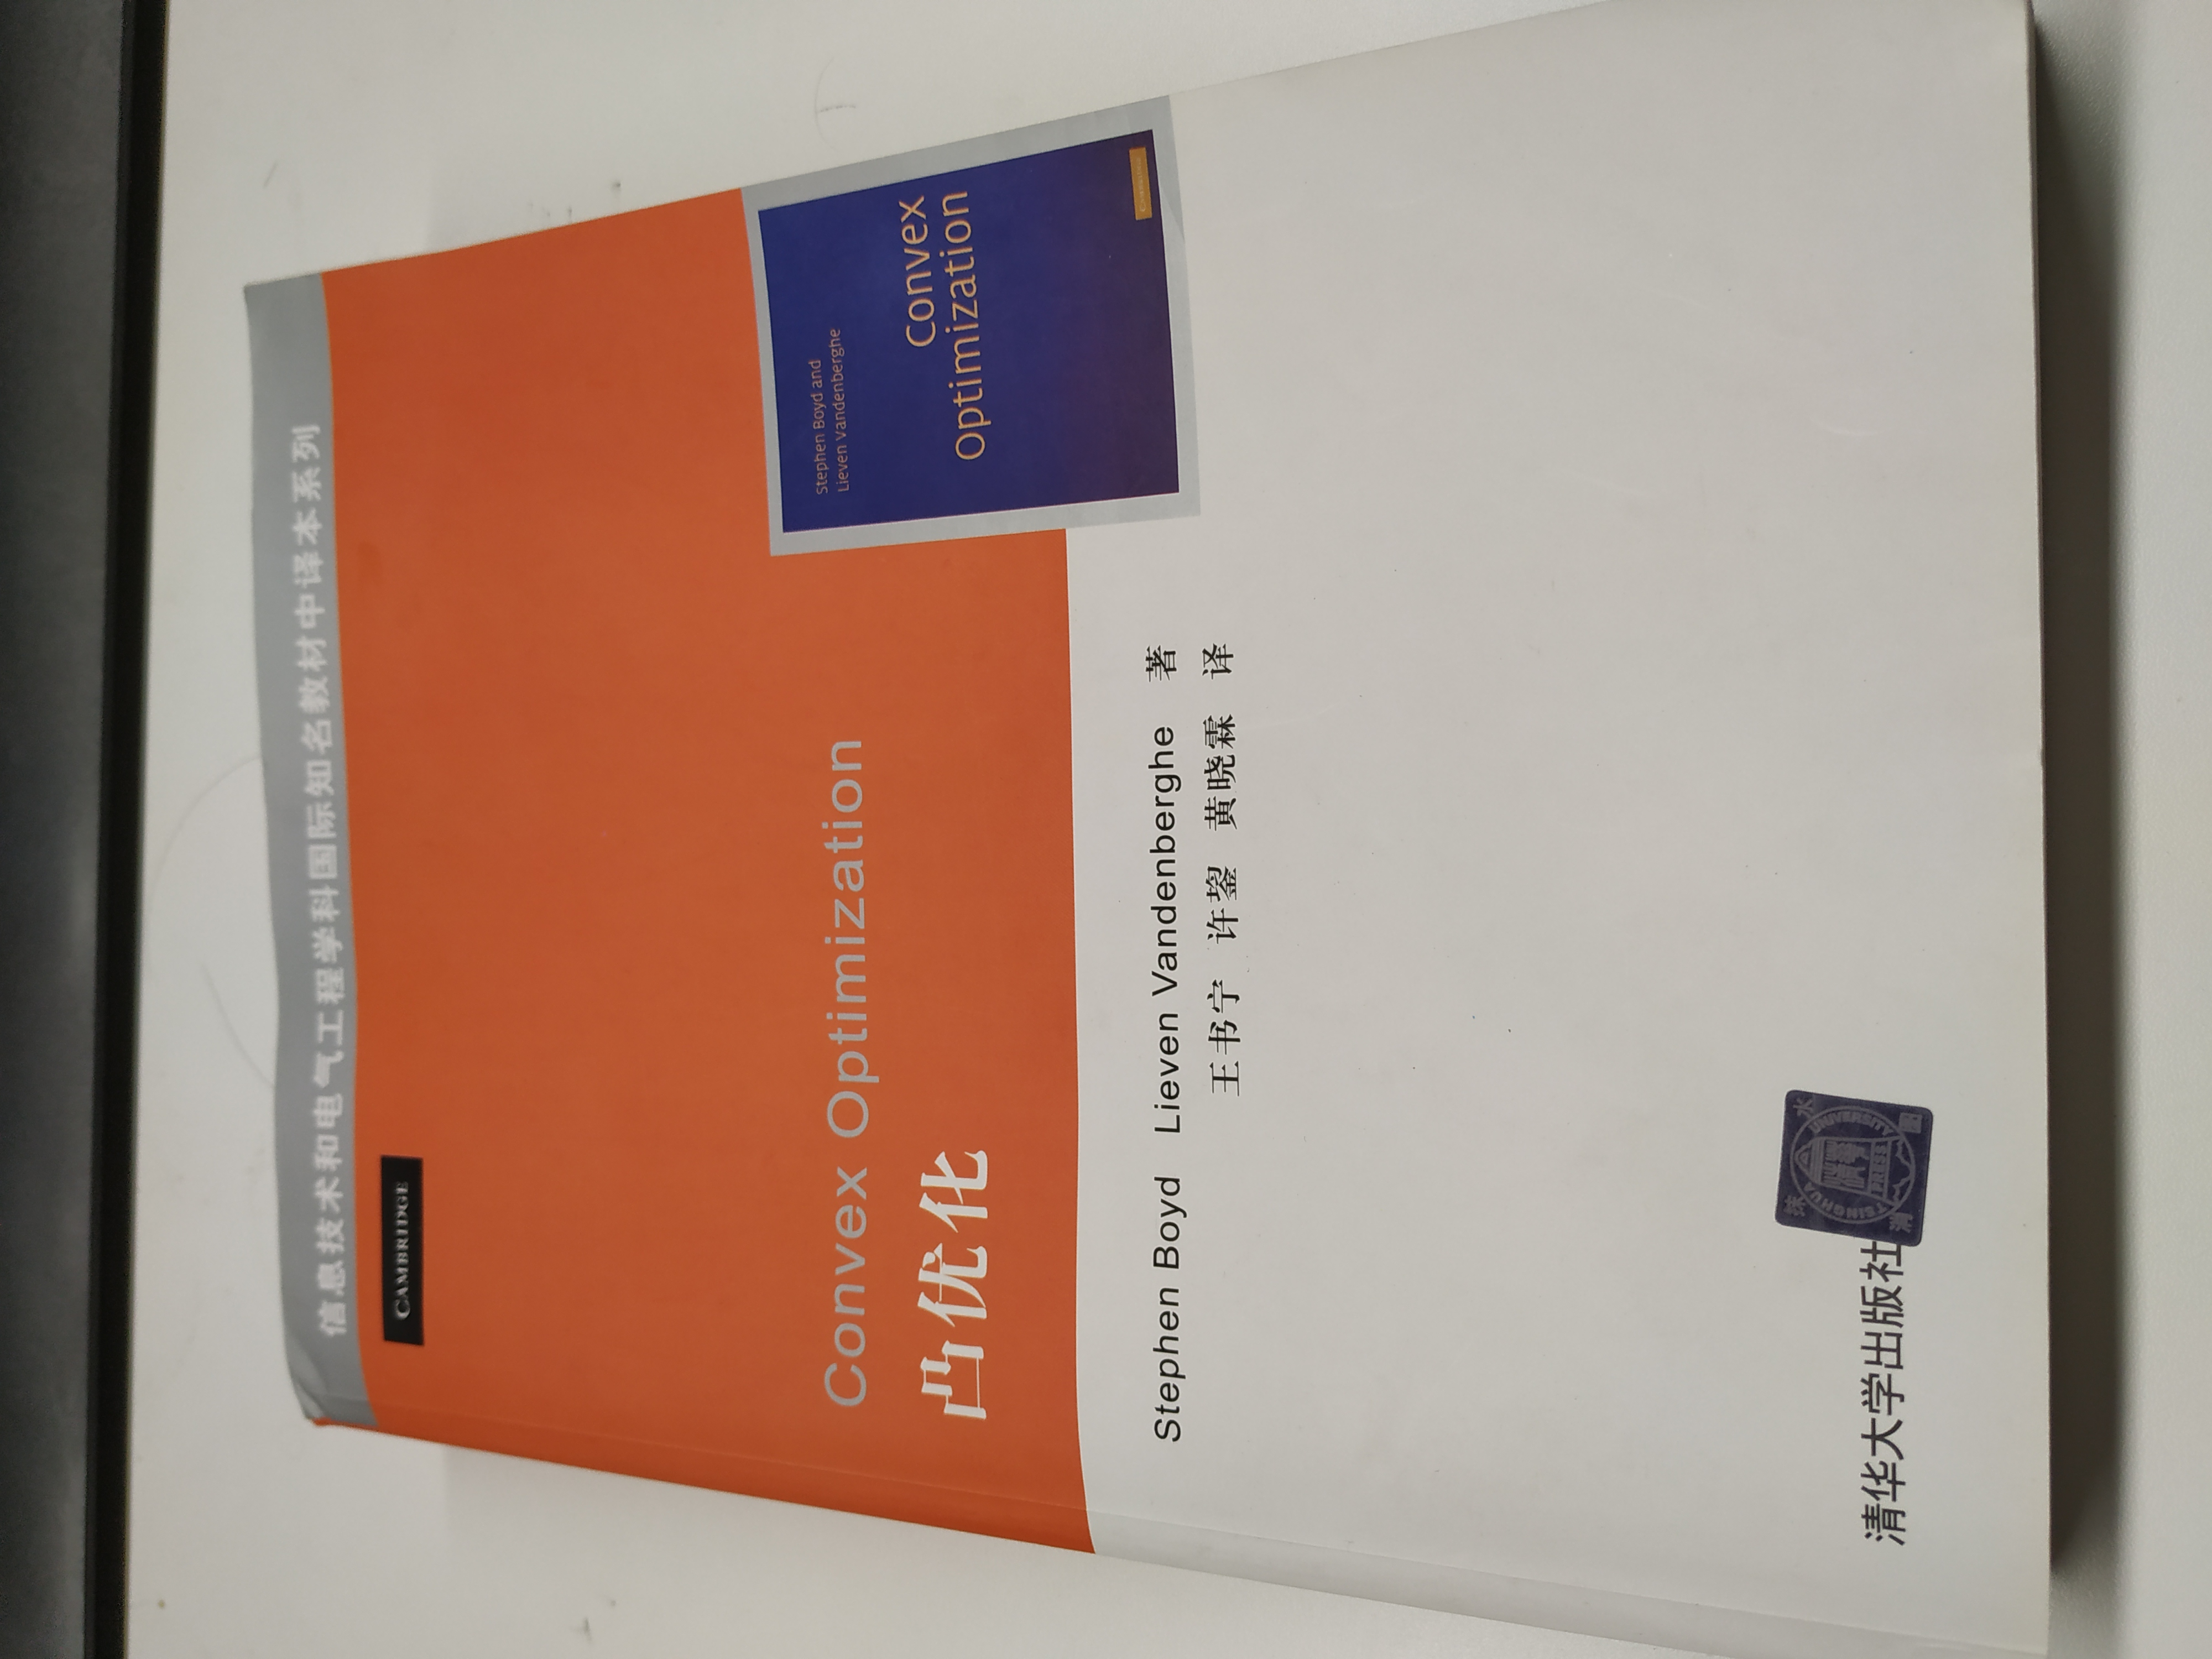
\includegraphics[scale=0.1]{amcl/tyh.jpg}
%     % 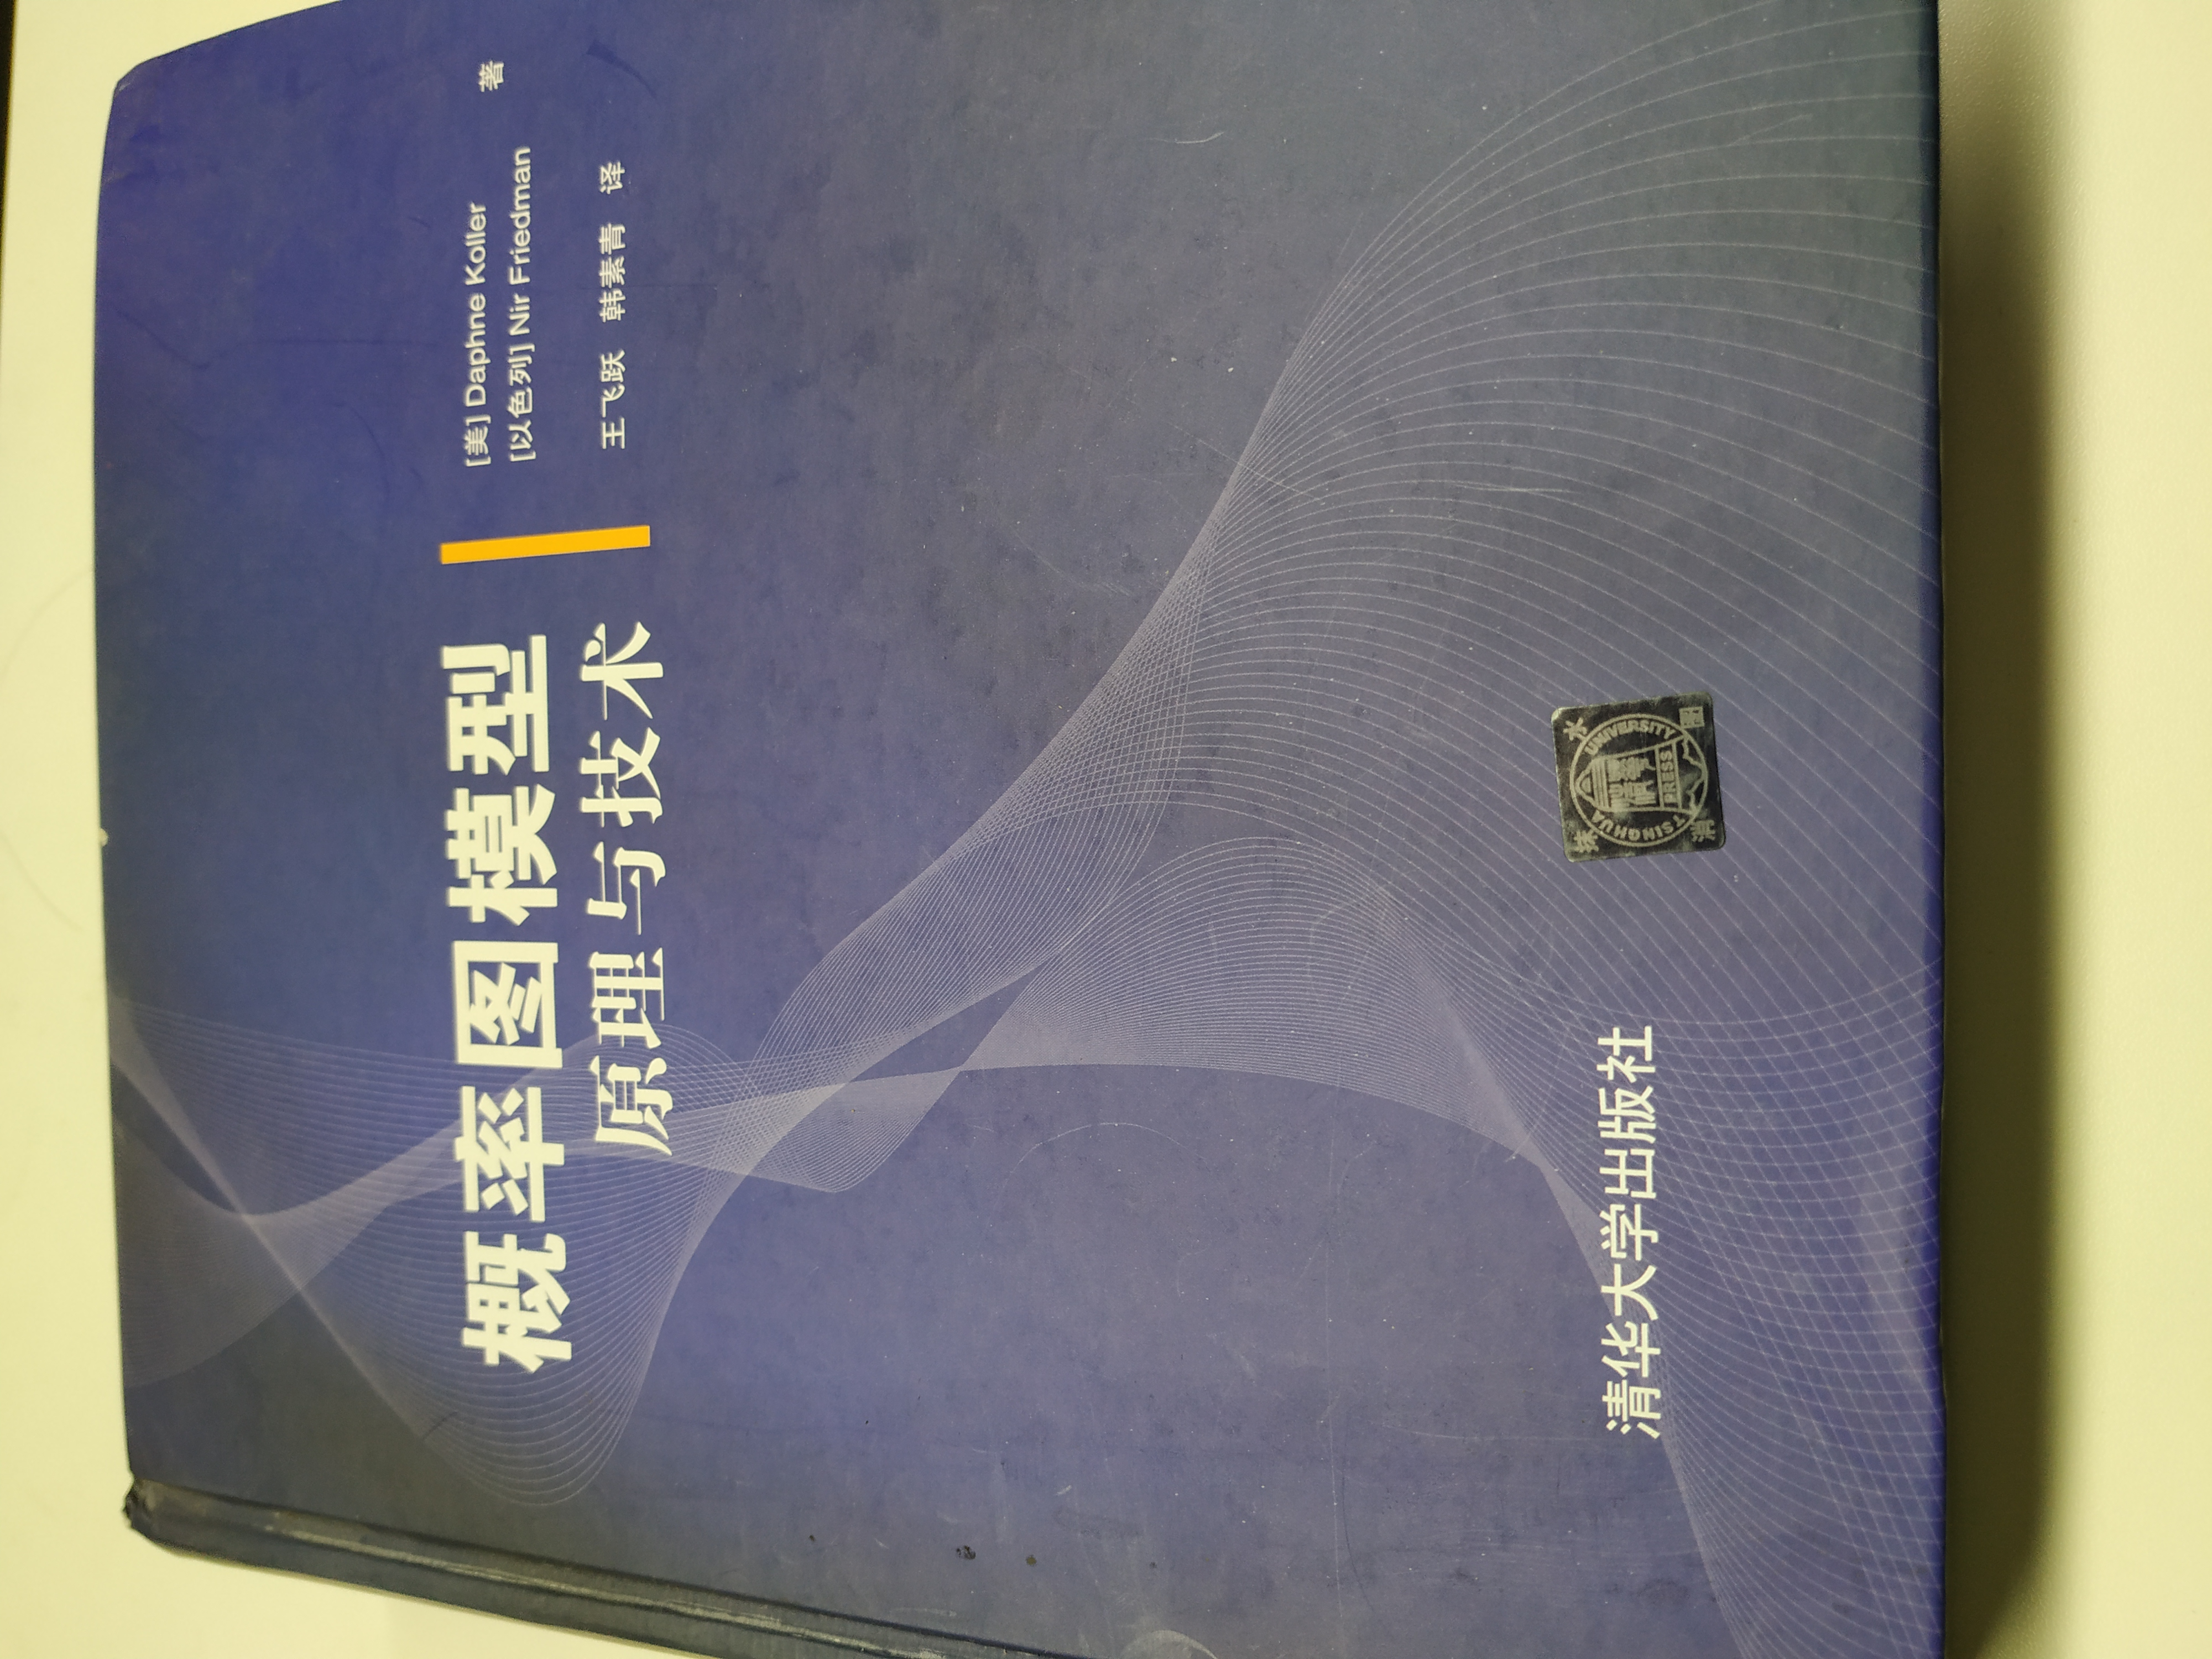
\includegraphics[height=3.0cm]{amcl/gltmx.jpg}
    
%     % 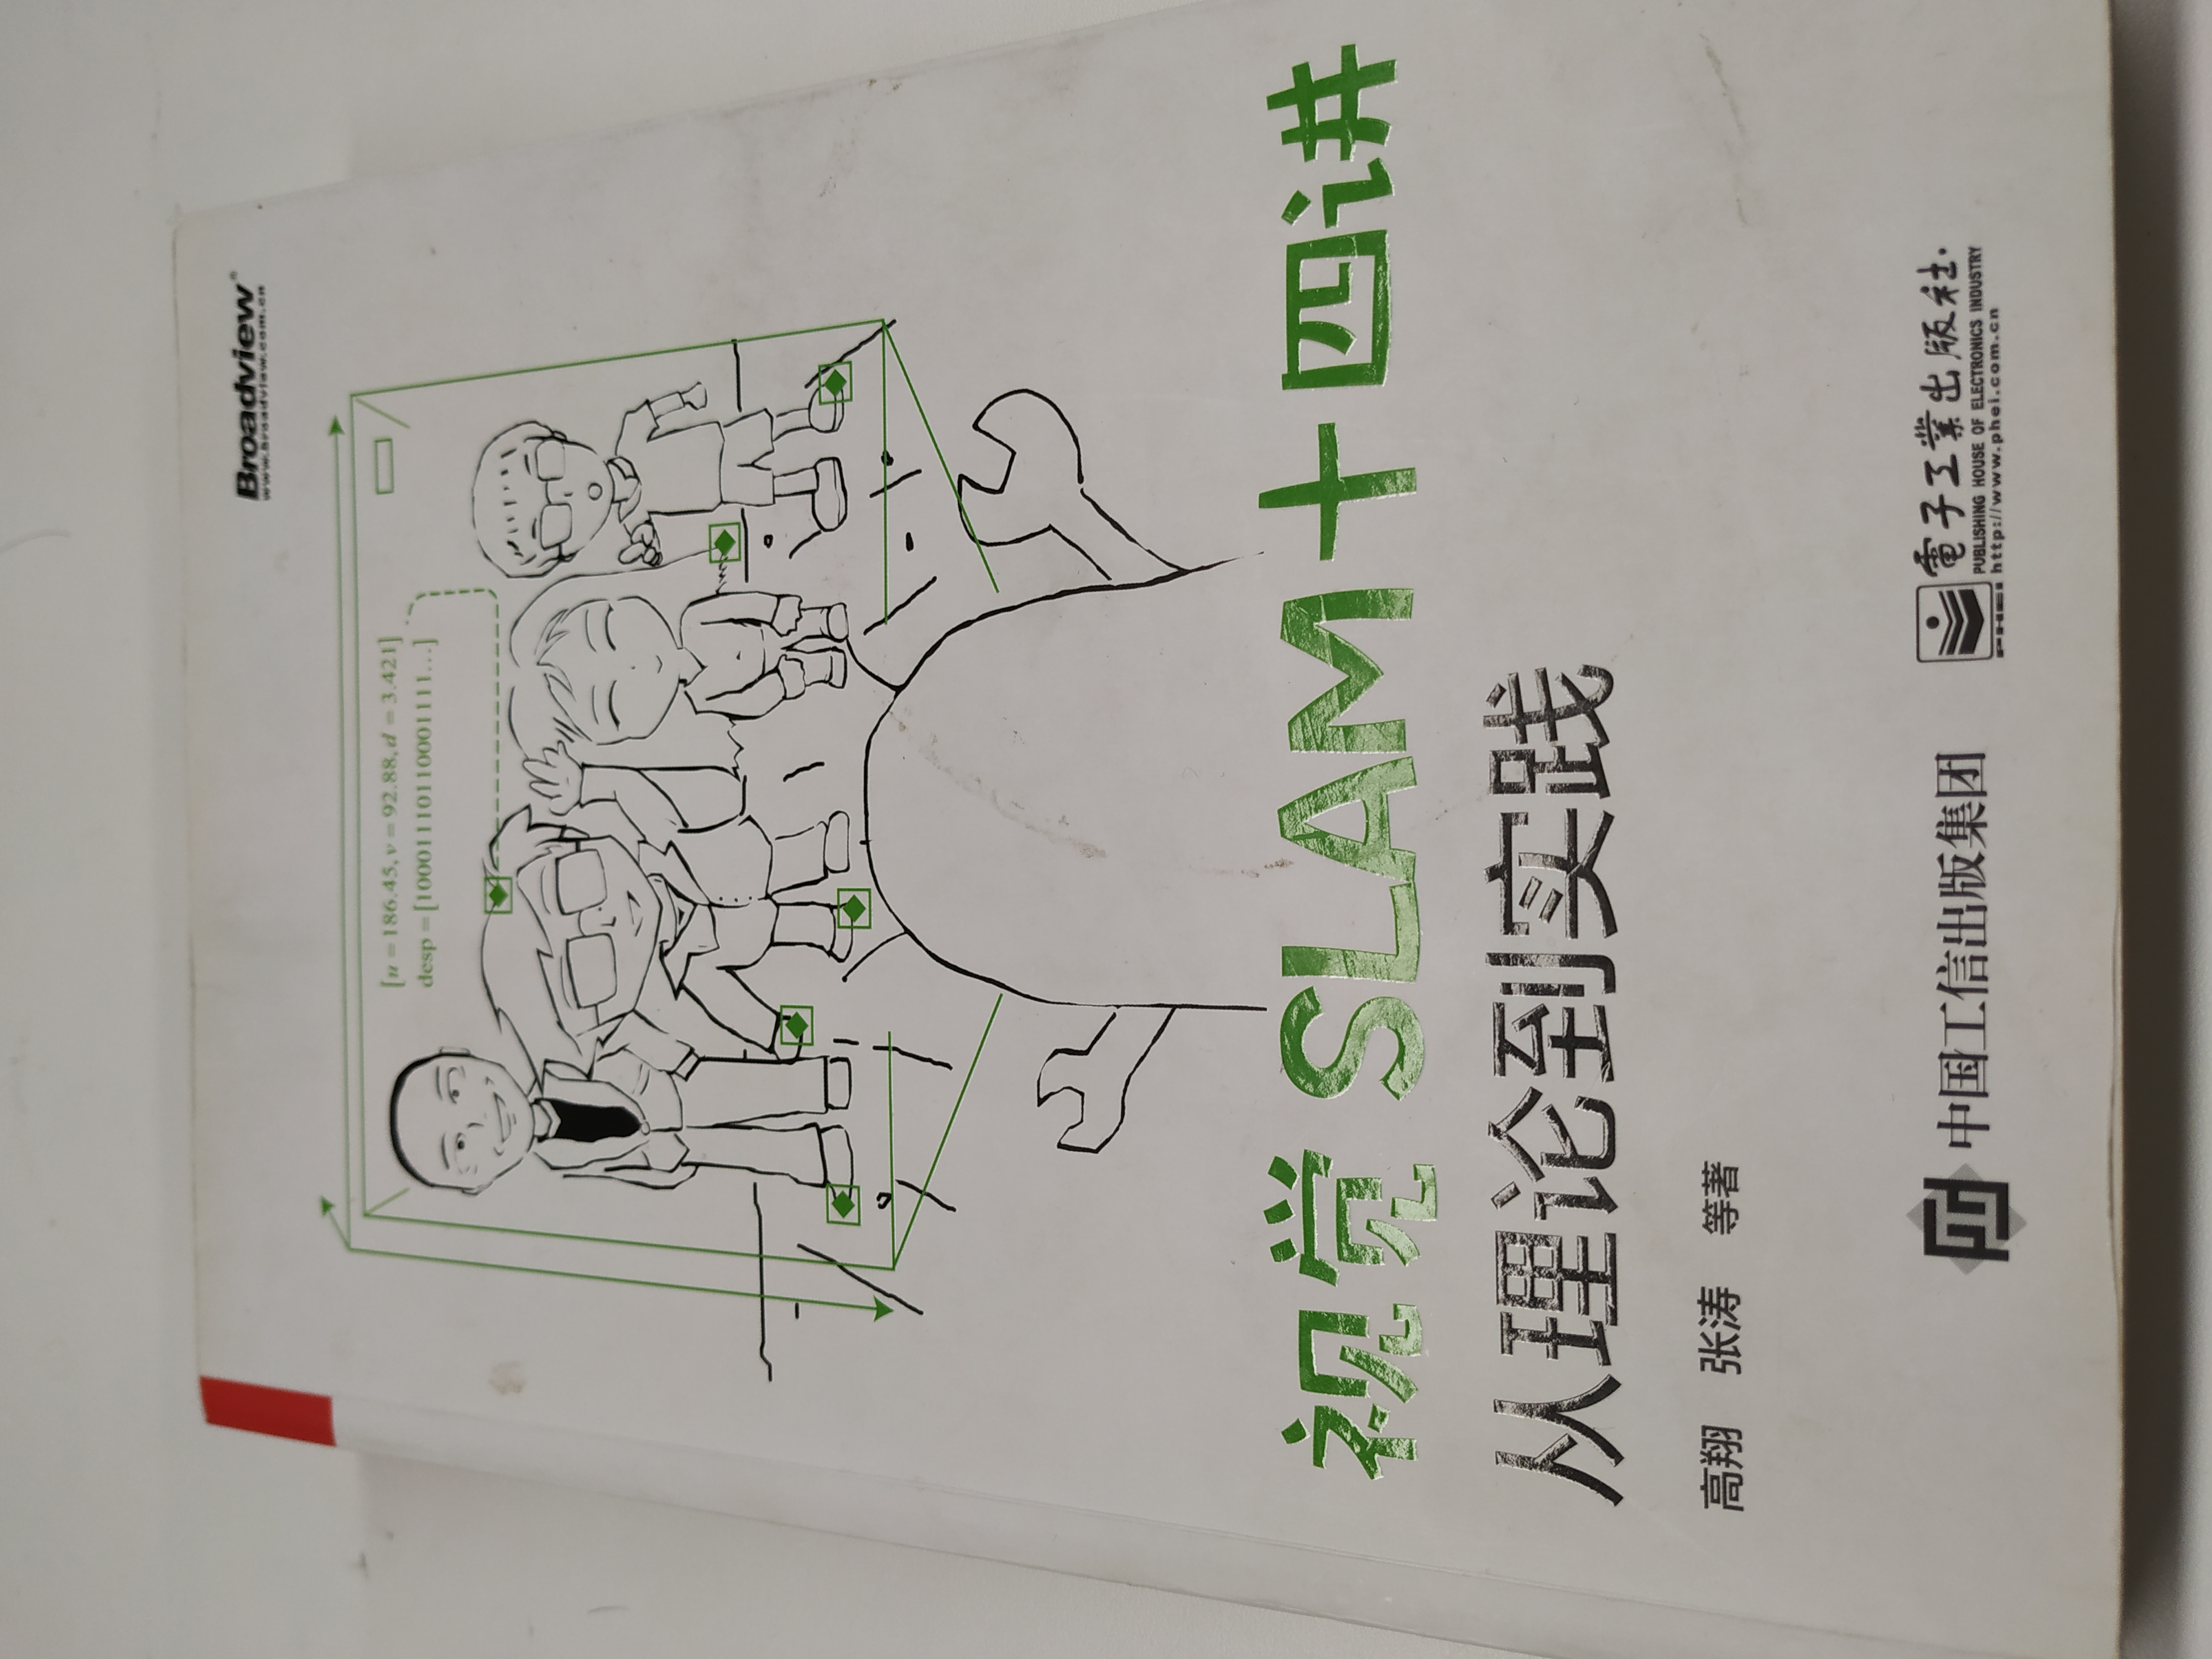
\includegraphics[height=3.0cm]{amcl/sjssj.jpg}
%     % 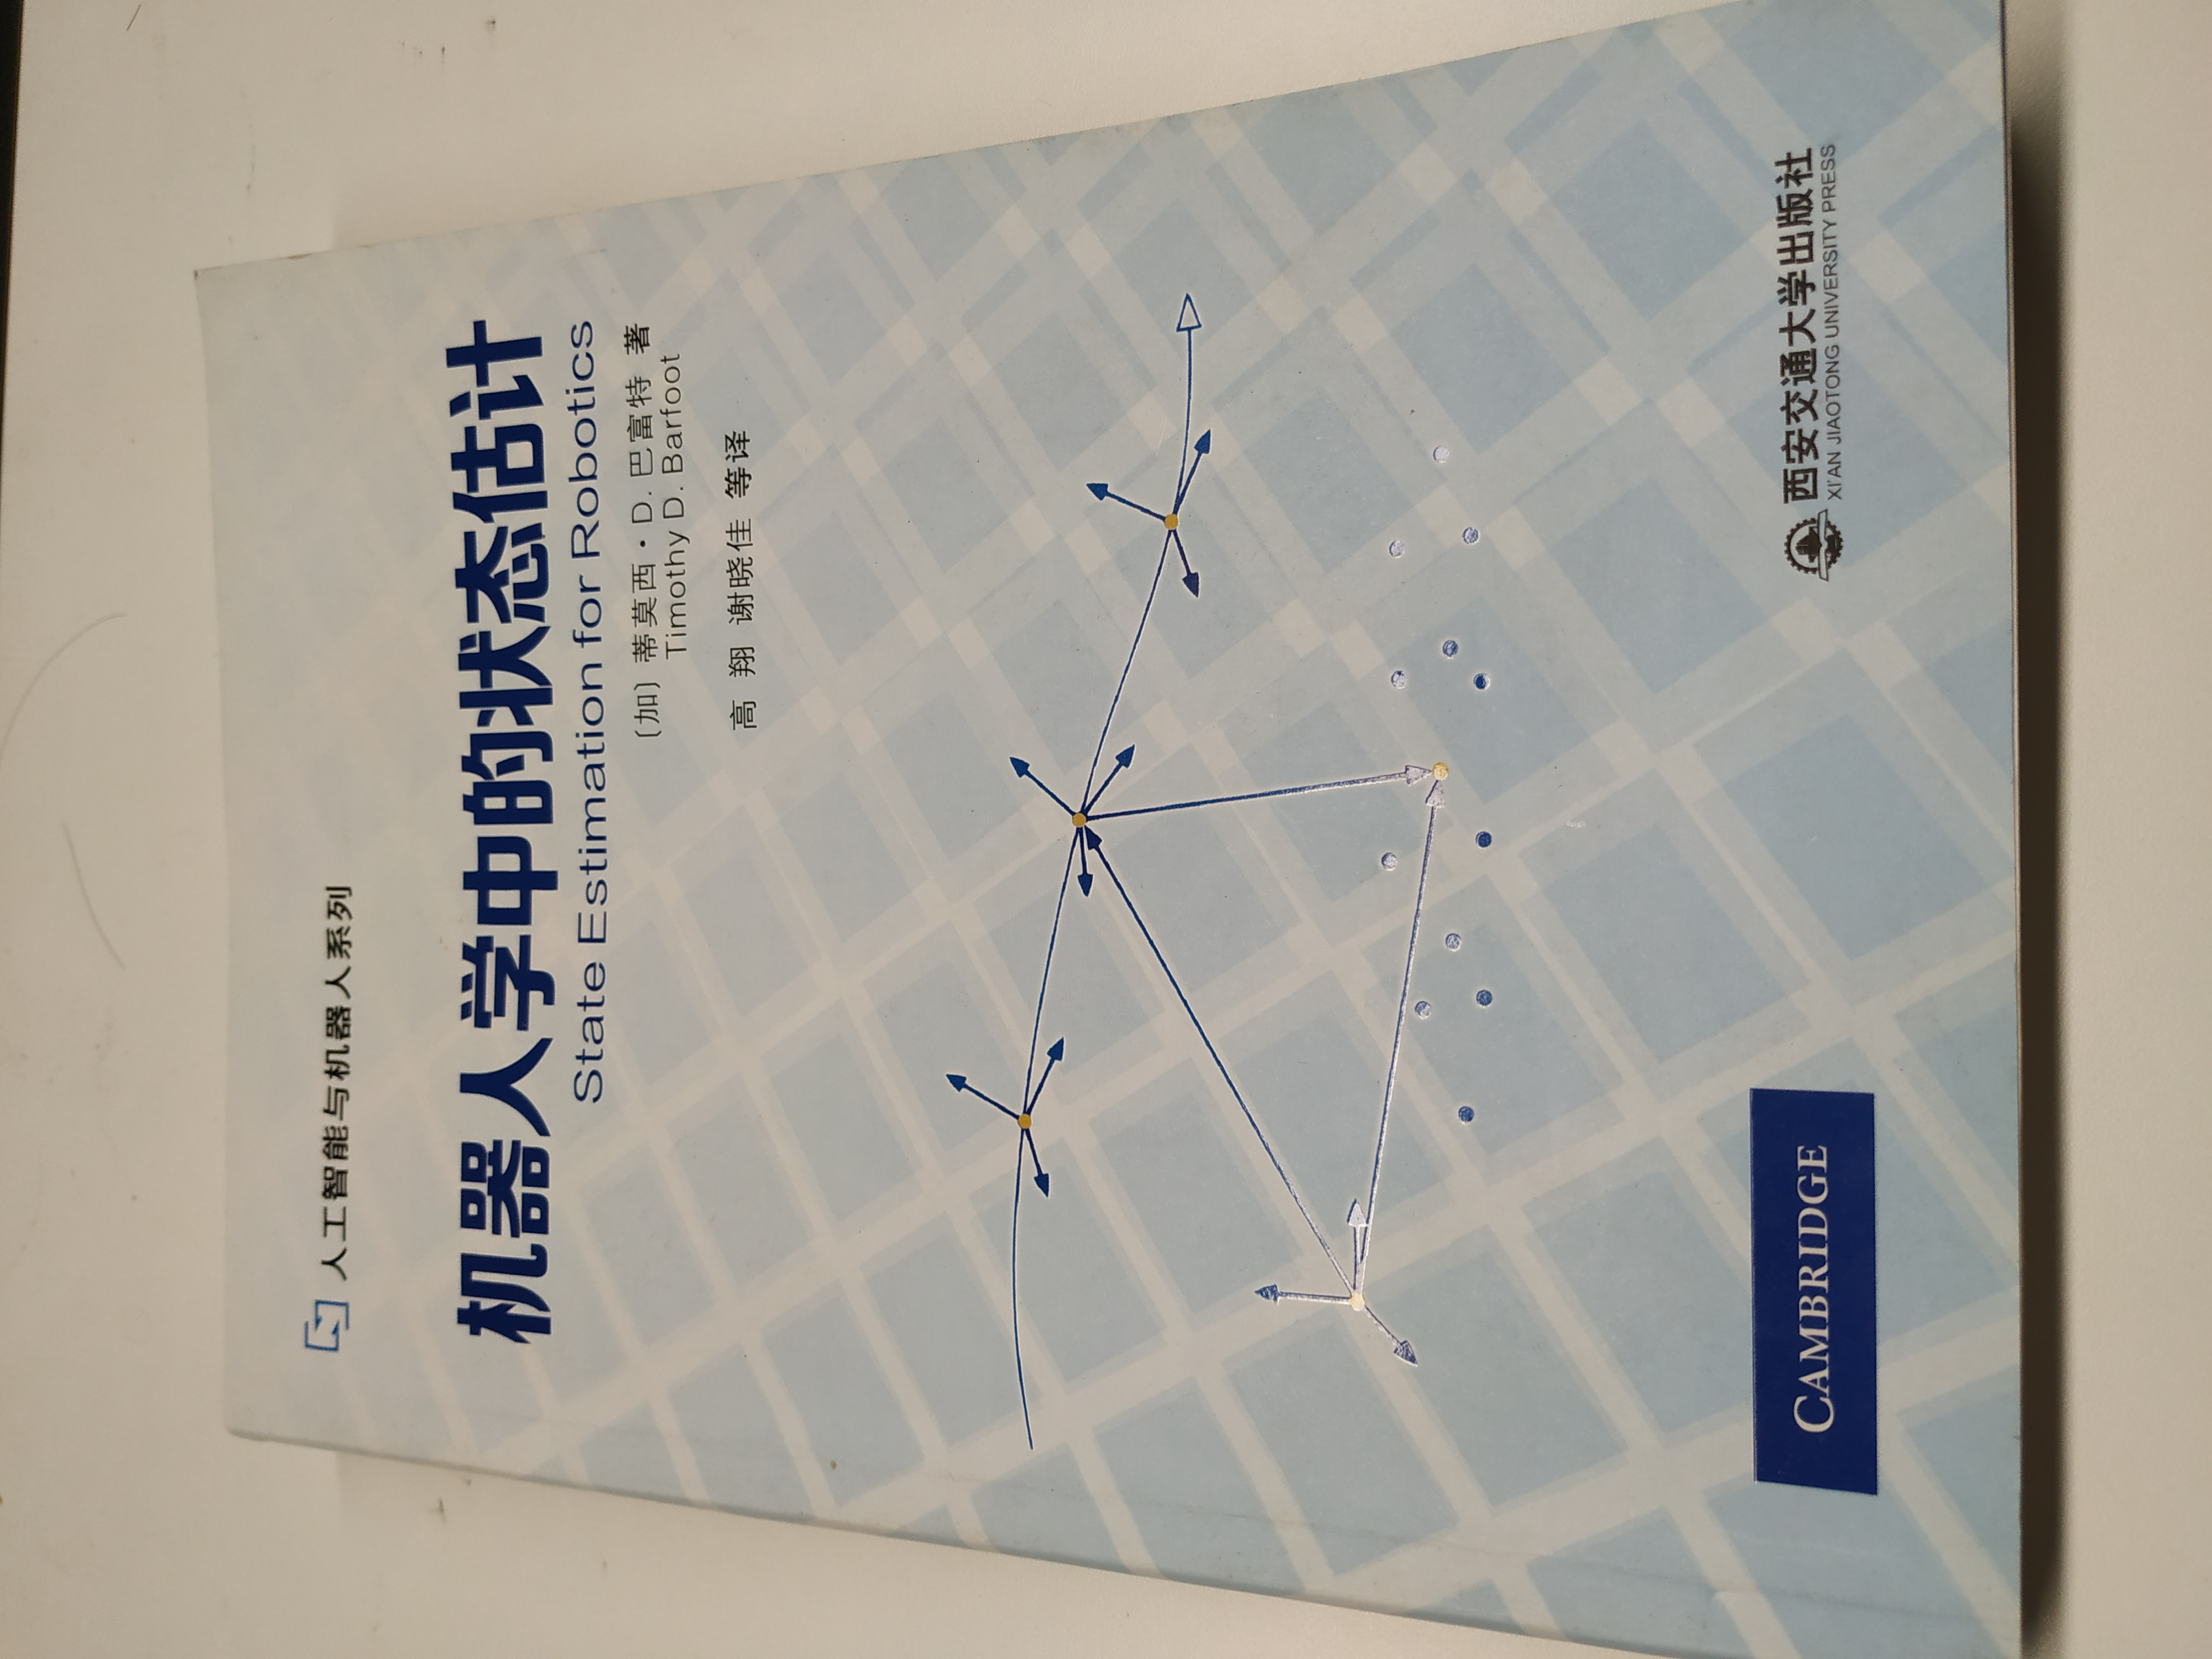
\includegraphics[height=3.0cm]{amcl/jqr.jpg}
%   \end{figure}
% \end{frame}